\chapter{测试与结果分析}

\section{实验环境与证据材料}
本文实验使用 IXI T1 脑部 MRI 数据作为主要数据来源。原始数据为 NIfTI 体数据，预处理后被转换为 PNG 二维切片，随后再打包为 StyleGAN2 训练数据集。根据训练配置文件，StyleGAN2 使用的数据集为 \texttt{mri128.zip}，最大训练切片数量为 60815 张，图像分辨率为 $128\times128$。

3DGS 实验使用连续 MRI 切片序列作为三维训练输入。训练集包含 180 张 $256\times256$ 切片，系统使用 300000 个初始点作为三维高斯优化起点。上述设置均可在项目训练目录中的相机参数、输入点云和训练日志中查到。

本章尽量用项目中已经保存的文件说明实验结果。训练配置、日志文件、模型权重、生成切片、点云文件、3DGS checkpoint、渲染图像和指标统计结果都来自项目源码目录和结果目录。这些材料可以对应到数据处理、二维生成、三维重建和平台测试等环节，也方便后续复核。

\begin{table}[H]
\centering
\caption{实验与测试证据材料}
\begin{tabular}{>{\raggedright\arraybackslash}p{4.1cm}>{\raggedright\arraybackslash}p{6.4cm}p{2.1cm}}
\toprule
证据材料 & 项目路径 & 状态 \\
\midrule
StyleGAN2 训练配置 & \thesispath{results/training_runs/00000-.../training_options.json} & 已确认 \\
StyleGAN2 训练日志 & \thesispath{results/training_runs/00000-.../log.txt} & 已确认 \\
可加载模型权重 & \thesispath{results/training_runs/network-snapshot-010000.pkl} & 已确认 \\
训练样本网格 & \thesispath{results/training_runs/00000-.../reals.png} & 已确认 \\
生成切片示例 & \thesispath{results/generated_slices/seed0042.png} 等 & 已确认 \\
初始点云文件 & \thesispath{results/3d_model_test/init_point_cloud.ply} & 已确认 \\
3DGS 训练日志 & \thesispath{results/3dgs_runs/mri_bestcand80_.../train.log} & 已确认 \\
3DGS 模型权重 & \thesispath{results/3dgs_runs/mri_bestcand80_.../chkpnt30000.pth} & 已确认 \\
3DGS 输出点云 & \thesispath{results/3dgs_runs/mri_bestcand80_.../point_cloud/iteration_30000/point_cloud.ply} & 已确认 \\
3DGS 渲染结果 & \thesispath{results/3dgs_runs/mri_bestcand80_.../train/ours_30000/renders} & 已确认 \\
\bottomrule
\end{tabular}
\end{table}

\section{StyleGAN2 训练配置与结果}
StyleGAN2 训练采用单 GPU 配置。Batch size 设置为 4，配置训练量为 25000 kimg。生成器和判别器均使用 Adam 优化器，学习率为 0.0025。潜变量维度和中间潜变量维度均为 512。训练过程中启用 ADA 数据增强，目标值为 0.6。训练输出目录保存训练配置、训练日志、真实样本网格和模型权重快照。

\begin{table}[H]
\centering
\caption{StyleGAN2 训练主要参数}
\begin{tabular}{p{4cm}p{8cm}}
\toprule
参数项 & 参数值 \\
\midrule
训练数据 & \texttt{mri128.zip} \\
图像分辨率 & $128\times128$ \\
训练切片数量 & 60815 \\
GPU 数量 & 1 \\
Batch Size & 4 \\
配置训练量 & 25000 kimg \\
模型快照 & \texttt{network-snapshot-010000.pkl} \\
优化器 & Adam \\
学习率 & 0.0025 \\
ADA 目标值 & 0.6 \\
\bottomrule
\end{tabular}
\end{table}

训练样本网格如图 \ref{fig:stylegan2-reals} 所示。该图来自训练输出目录中的 \texttt{reals.png}，可用于确认训练集是否被正确读取。样本网格中的输入样本为单通道脑部 MRI 切片，图中可以看到脑部轮廓和灰度层次。从实验观察看，预处理后的切片灰度范围较稳定，能够作为二维生成模型的训练输入。

\begin{figure}[H]
\centering
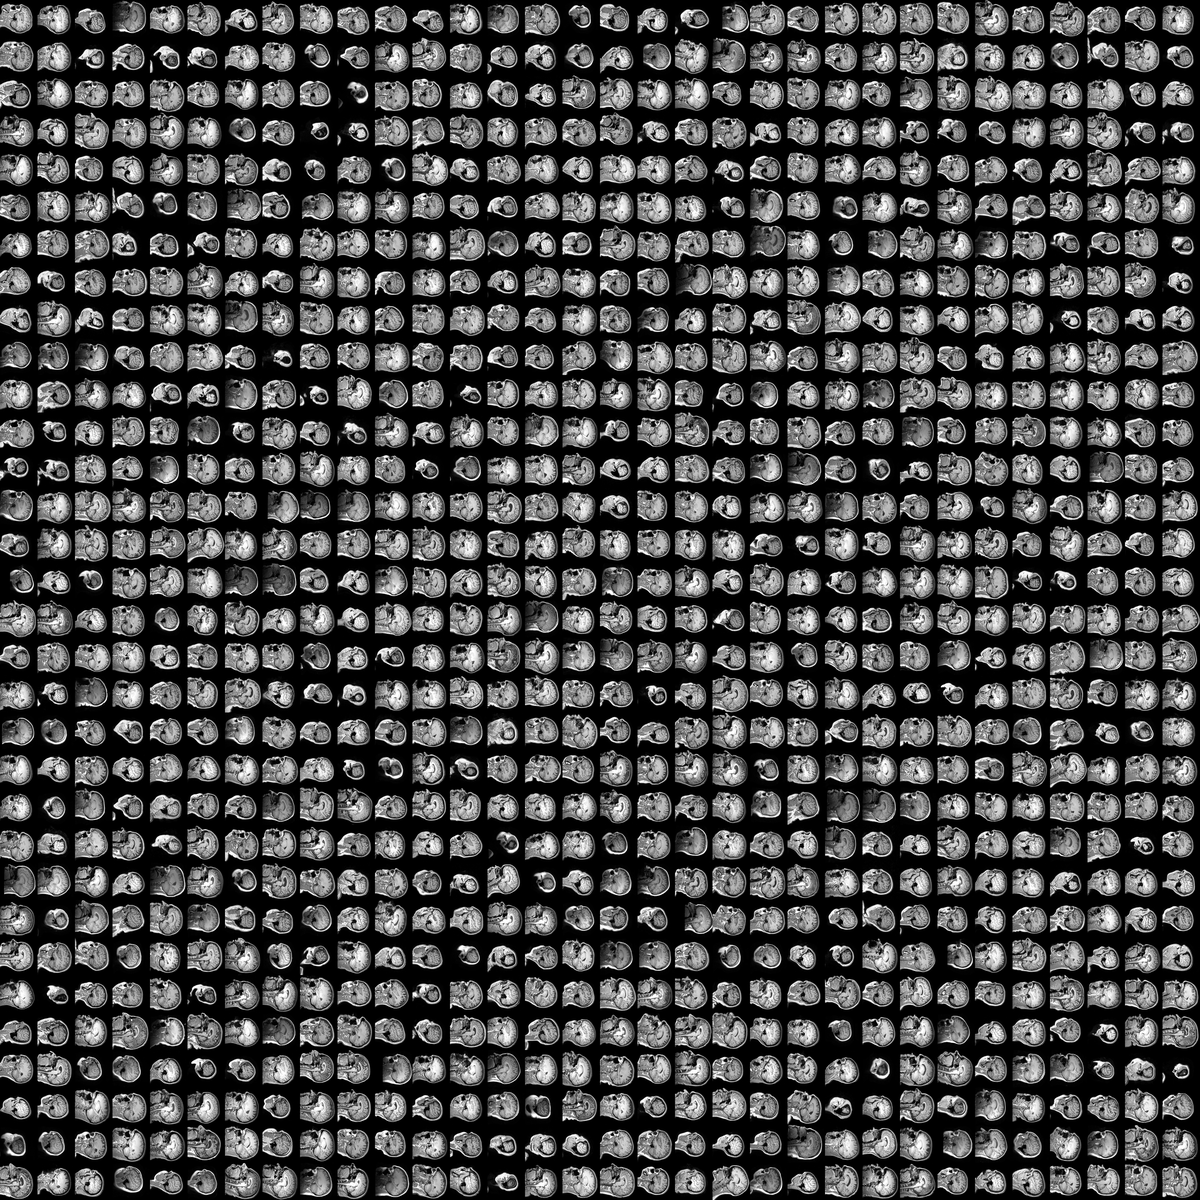
\includegraphics[width=0.82\textwidth]{figures/stylegan2_reals_preview.png}
\caption{StyleGAN2 训练集中真实 MRI 切片样本网格}
\label{fig:stylegan2-reals}
\end{figure}

训练结束后，项目得到可加载的模型快照 \texttt{network-snapshot-010000.pkl}。平台能够读取该权重并生成 MRI 切片，说明权重加载、潜变量采样、生成器推理、图像张量转换和 PNG 保存等环节可以顺利衔接。对 StyleGAN2 结果的评价不放在临床诊断性能上，而是关注生成链路是否可用、输出是否可复现，以及生成切片能否继续支撑三维输入组织。

\section{二维切片生成结果分析}
平台生成的示例切片如图 \ref{fig:generated-slices} 所示。图像来自生成切片结果目录，由训练完成的 StyleGAN2 权重生成。不同随机种子对应不同潜变量输入，因此输出切片在灰度分布和结构形态上会出现差异。图中可以看到脑部 MRI 切片的基本轮廓和灰度层次，这说明平台推理模块能够正确调用训练权重，并把模型输出保存为可查看的图像结果。

\begin{figure}[H]
\centering
\begin{subfigure}{0.32\textwidth}
\centering
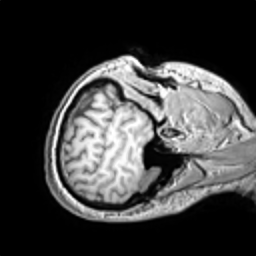
\includegraphics[width=\textwidth]{figures/generated_seed0123.png}
\caption{随机种子 123}
\end{subfigure}
\hspace{0.08\textwidth}
\begin{subfigure}{0.32\textwidth}
\centering
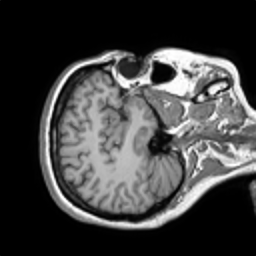
\includegraphics[width=\textwidth]{figures/generated_seed0042.png}
\caption{随机种子 42}
\end{subfigure}
\caption{StyleGAN2 生成的 MRI 切片示例}
\label{fig:generated-slices}
\end{figure}

从操作流程看，二维切片生成已经可以在平台中闭环完成。用户指定模型权重、生成数量、截断参数和随机种子后，后端完成潜变量采样、生成器推理、灰度图像转换和结果保存。截断参数 \texttt{truncation\_psi} 会影响图像稳定性和变化幅度，随机种子则保证同一参数下能够再次生成相同结果。该功能既能提供论文展示图，也能为连续切片序列和点云初始化提供输入。

\section{平台功能测试}
平台功能测试关注主要流程是否按预期运行。测试内容包括 FastAPI 后端接口、React 前端页面、数据预处理、模型训练入口、切片生成、连续序列生成、点云初始化、3DGS 结果展示和 AI 助手。测试结果显示，FastAPI 后端服务可以正常启动，React 前端可以访问平台页面；生成模块能够调用训练完成的权重输出 PNG 切片；点云初始化模块能够从切片目录生成 PLY 文件；3DGS 训练结果也能够以日志、渲染图像和点云文件形式归档。

\begin{table}[H]
\centering
\caption{平台主要功能测试结果}
\begin{tabular}{>{\raggedright\arraybackslash}p{3cm}>{\raggedright\arraybackslash}p{5.2cm}>{\raggedright\arraybackslash}p{4.8cm}}
\toprule
测试模块 & 测试内容 & 测试结果 \\
\midrule
数据预处理 & NIfTI 读取、轴向切片、归一化、缩放和 PNG 保存 & 已实现，可按数据目录批量处理 \\
模型训练 & 自动识别训练数据并启动 StyleGAN2 训练 & 已实现，训练结果已存在 \\
切片生成 & 加载 \texttt{.pkl} 权重并生成 PNG 图像 & 已通过，已有生成样例 \\
连续序列 & 潜空间插值得到连续切片序列 & 已实现，可用于三维展示 \\
点云初始化 & 将切片序列转换为 PLY 点云 & 已通过，已有 PLY 结果 \\
3DGS 重建 & 组织切片、点云、相机参数并完成训练输出 & 已通过，已有 checkpoint、点云和渲染结果 \\
FastAPI 后端 & 提供概览、生成、资产、任务、分析、报告和 AI 助手接口 & 已实现，可由 React 前端调用 \\
React 前端 & 提供仪表盘、生成、查看器、影像分析报告、可信性评估、任务、3D 和教学页面 & 已实现，可通过 Vite 本地服务访问 \\
AI 助手 & 参数说明和平台问答 & 已实现，包含本地解释逻辑和可选搜索接口 \\
\bottomrule
\end{tabular}
\end{table}

测试过程显示，平台已经具备毕业设计展示和实验复核所需的几项核心能力。第一，用户可以通过 React 前端生成二维切片并查看输出结果。第二，平台可以浏览连续 MRI 切片，并进入点云或体渲染页面查看三维资产。第三，FastAPI 后端可以维护任务状态、结果路径和日志信息，前端页面不需要直接调用底层训练脚本。第四，系统能够给出可信性提示和影像分析报告，用于说明生成结果的使用边界。需要说明的是，这些提示和报告只服务于教学解释与结果整理，不作为临床诊断依据。

为了更直观地展示平台实现效果，本文选取系统总览页、生成工作台、医学影像查看器和三维点云展示页作为功能截图。系统总览页汇总生成切片数量、连续序列数量、三维资产数量和当前风险提示状态，如图 \ref{fig:frontend-dashboard-generation}（a）所示。生成工作台用于配置模型权重、随机种子、截断参数和生成数量，并通过 FastAPI 后端调用 StyleGAN2 生成模块，如图 \ref{fig:frontend-dashboard-generation}（b）所示。这两个页面展示了平台从状态查看到二维切片生成的主要操作路径。

\begin{figure}[H]
\centering
\begin{subfigure}{0.48\textwidth}
\centering
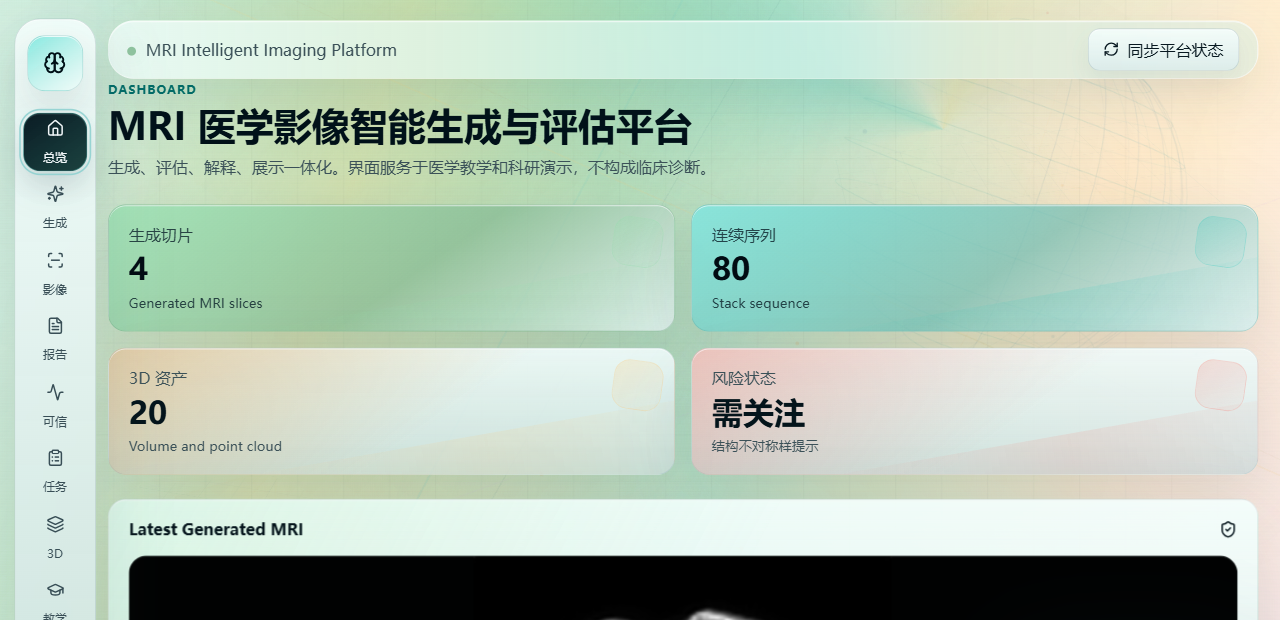
\includegraphics[width=\textwidth]{figures/frontend_dashboard.png}
\caption{系统总览页}
\end{subfigure}
\hfill
\begin{subfigure}{0.48\textwidth}
\centering
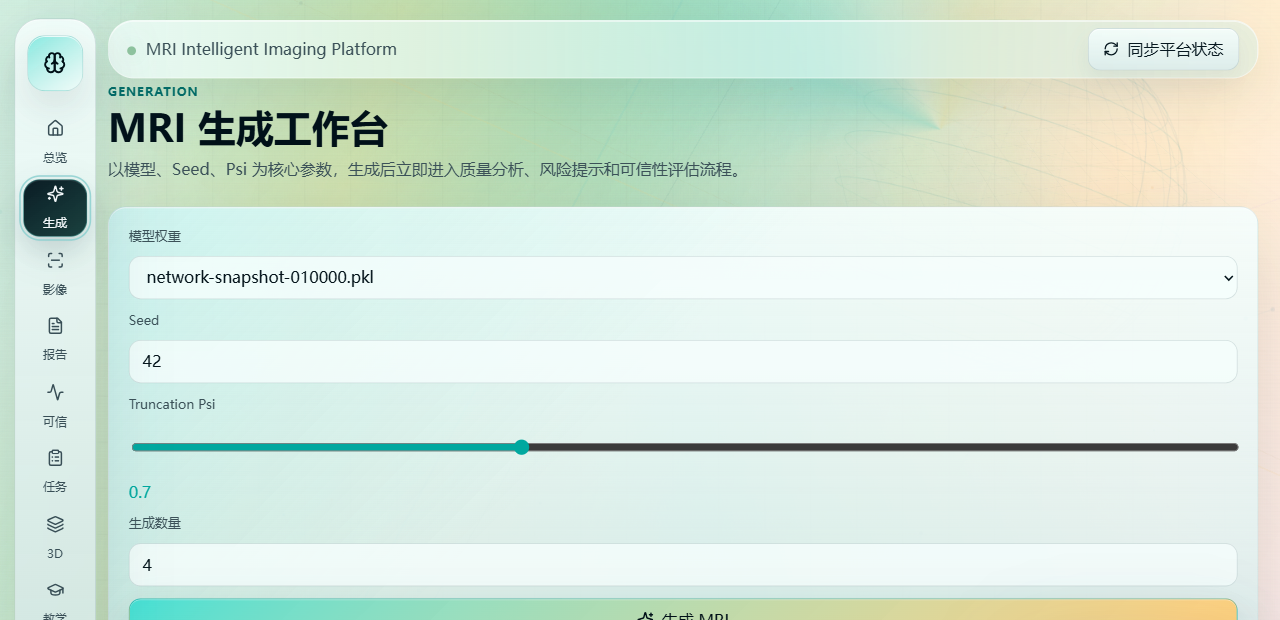
\includegraphics[width=\textwidth]{figures/frontend_generation.png}
\caption{生成工作台}
\end{subfigure}
\caption{React 前端系统总览与生成工作台页面}
\label{fig:frontend-dashboard-generation}
\end{figure}

医学影像查看器和三维点云展示页主要用于结果复核。医学影像查看器基于前端影像组件显示连续 MRI 切片，并提供窗位、窗宽、缩放和平移等交互能力，如图 \ref{fig:frontend-viewer-pointcloud}（a）所示。三维点云展示页用于加载 3DGS 或 PLY 结构资产，并以轻量化点云形式展示三维重建结果，如图 \ref{fig:frontend-viewer-pointcloud}（b）所示。通过这两个页面，用户可以从二维切片观察扩展到三维结构查看，较完整地展示本系统“生成、分析、三维表达和教学演示”的设计目标。

\begin{figure}[H]
\centering
\begin{subfigure}{0.48\textwidth}
\centering
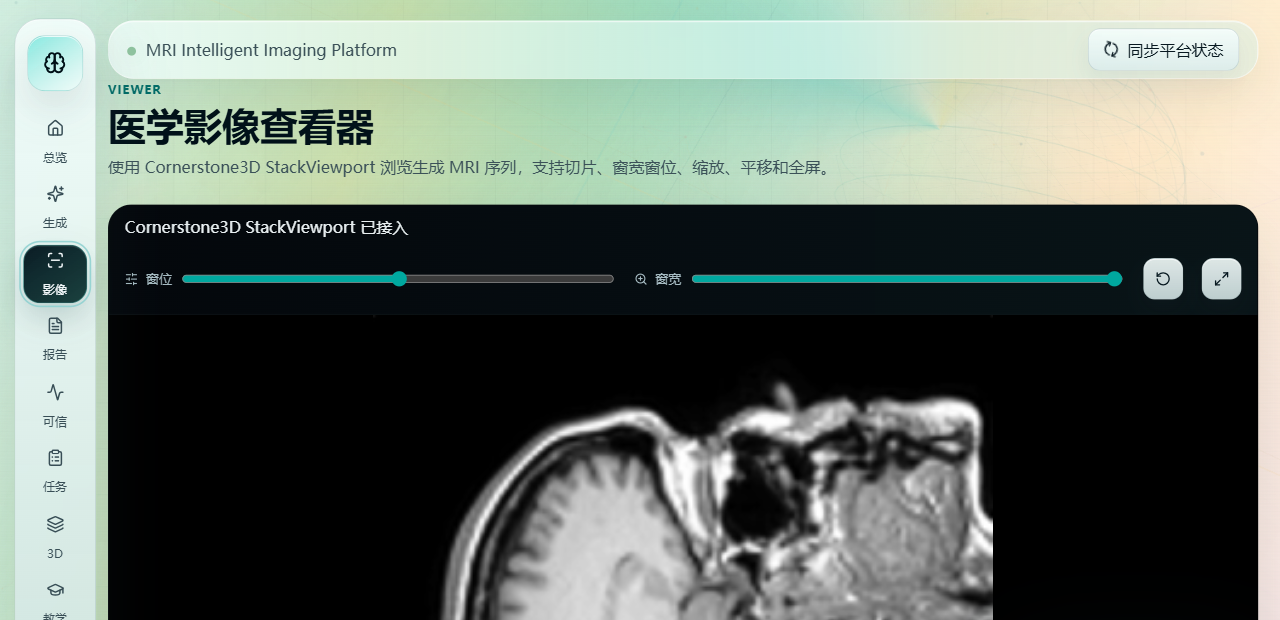
\includegraphics[width=\textwidth]{figures/frontend_viewer.png}
\caption{医学影像查看器}
\end{subfigure}
\hfill
\begin{subfigure}{0.48\textwidth}
\centering
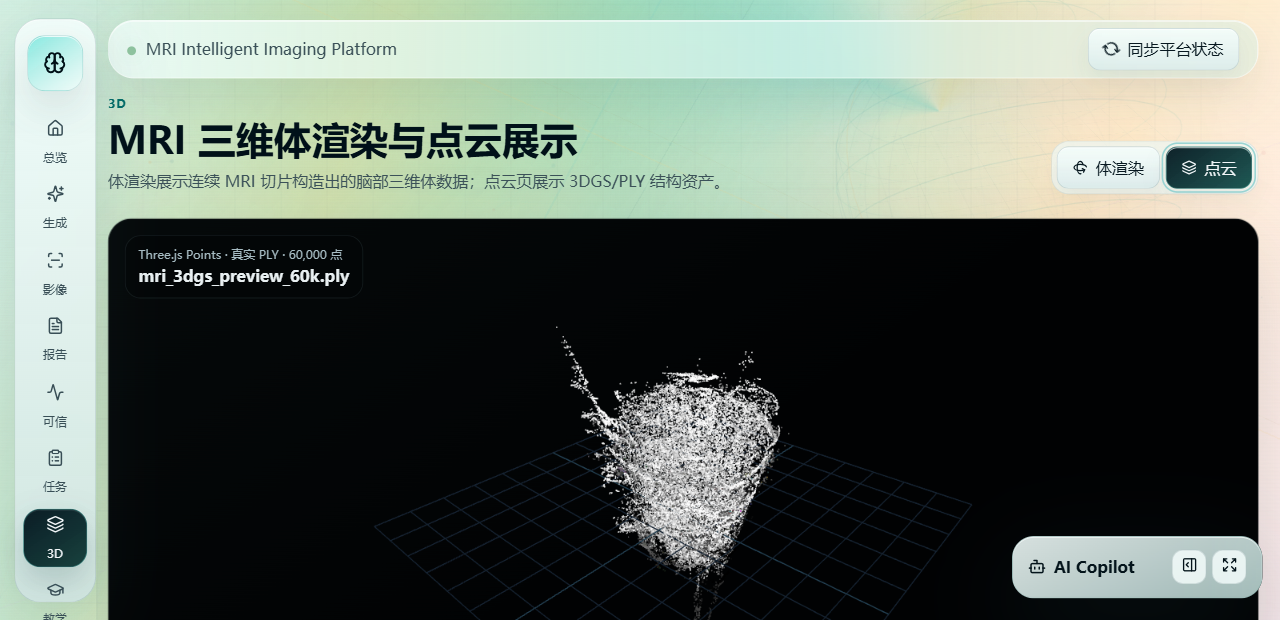
\includegraphics[width=\textwidth]{figures/frontend_pointcloud.png}
\caption{三维点云展示页}
\end{subfigure}
\caption{React 前端影像查看与三维点云展示页面}
\label{fig:frontend-viewer-pointcloud}
\end{figure}

三维页面还提供体渲染模式。该模式从连续 MRI 切片构建体数据，并通过阈值和透明度参数调节显示效果，如图 \ref{fig:frontend-volume} 所示。体渲染更适合观察连续切片形成的整体空间形态，点云模式则更适合展示 3DGS 或 PLY 结构资产。两种模式面向同一组三维结果，但观察侧重点不同。

\begin{figure}[H]
\centering
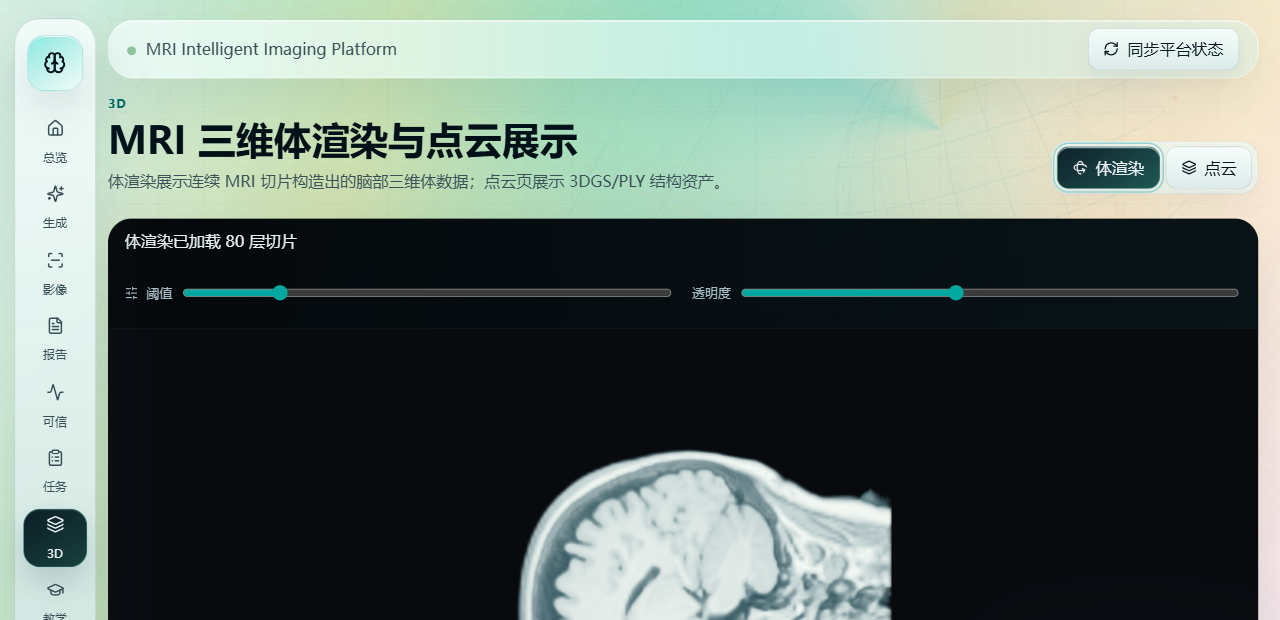
\includegraphics[width=0.82\textwidth]{figures/frontend_volume.png}
\caption{React 前端三维体渲染页面}
\label{fig:frontend-volume}
\end{figure}

报告页面和可信性评估页面用于解释生成结果。报告页面可以根据当前图像生成质量、结构、风险提示和教学说明，如图 \ref{fig:frontend-report-trust}（a）所示。可信性评估页面从真实性、多样性、非记忆性和解剖合理性等角度展示证据，如图 \ref{fig:frontend-report-trust}（b）所示。这两类页面不直接参与模型训练，但可以帮助用户理解生成结果的可靠性边界。

\begin{figure}[H]
\centering
\begin{subfigure}{0.48\textwidth}
\centering
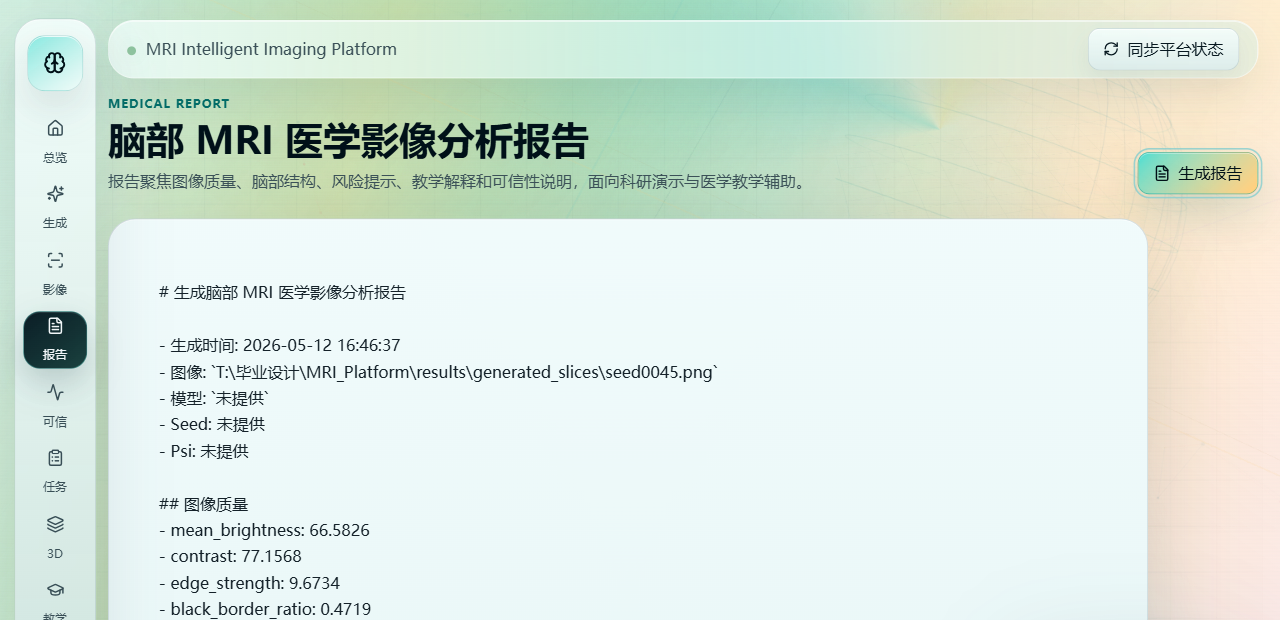
\includegraphics[width=\textwidth]{figures/frontend_report.png}
\caption{医学影像分析报告}
\end{subfigure}
\hfill
\begin{subfigure}{0.48\textwidth}
\centering
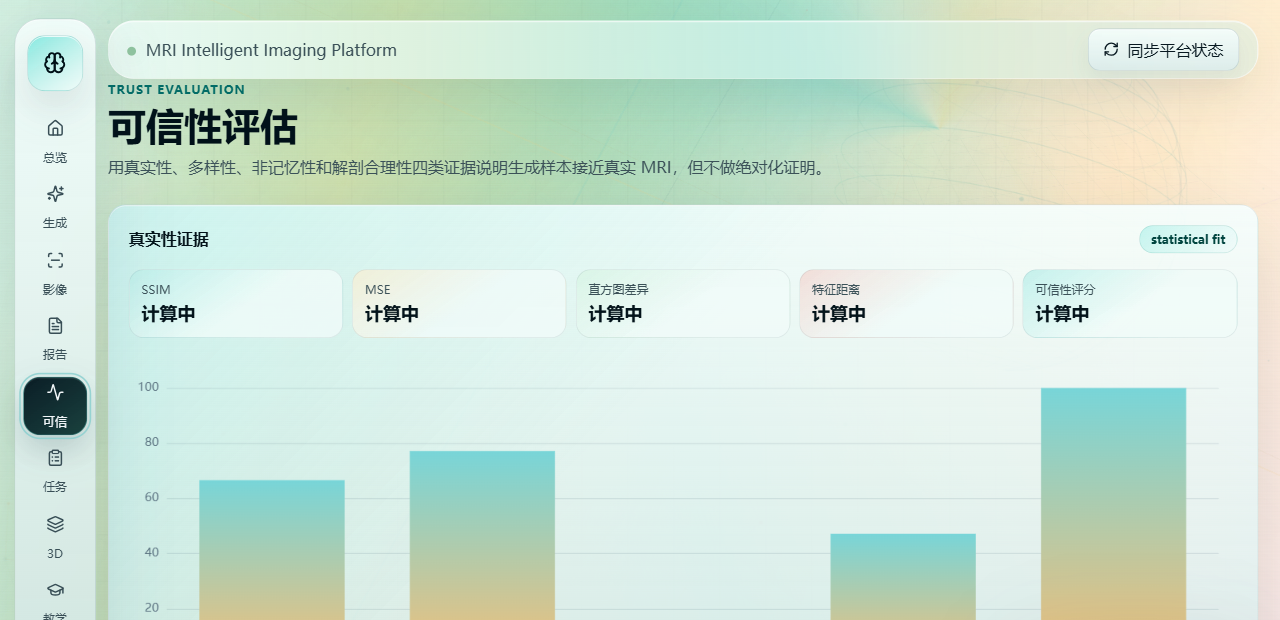
\includegraphics[width=\textwidth]{figures/frontend_trust.png}
\caption{可信性评估}
\end{subfigure}
\caption{React 前端报告生成与可信性评估页面}
\label{fig:frontend-report-trust}
\end{figure}

任务中心和医学教学中心用于支撑平台运行管理与答辩演示。任务中心记录生成、训练、评估、报告和三维任务的状态、输出路径和日志信息，如图 \ref{fig:frontend-tasks-education}（a）所示。医学教学中心把 MRI 基础、生成参数、质量指标和风险案例整理成交互式教学模块，如图 \ref{fig:frontend-tasks-education}（b）所示。通过这两个页面，系统不只展示算法结果，也能说明任务追踪、过程复核和教学辅助等工程功能。

\begin{figure}[H]
\centering
\begin{subfigure}{0.48\textwidth}
\centering
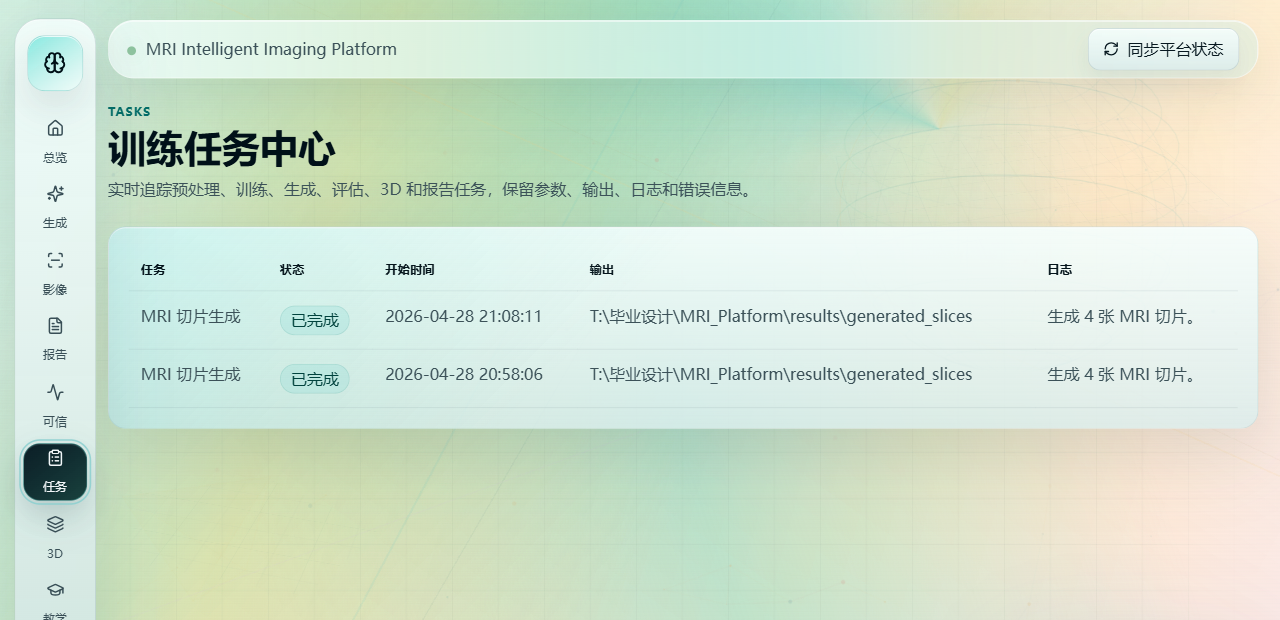
\includegraphics[width=\textwidth]{figures/frontend_tasks.png}
\caption{训练任务中心}
\end{subfigure}
\hfill
\begin{subfigure}{0.48\textwidth}
\centering
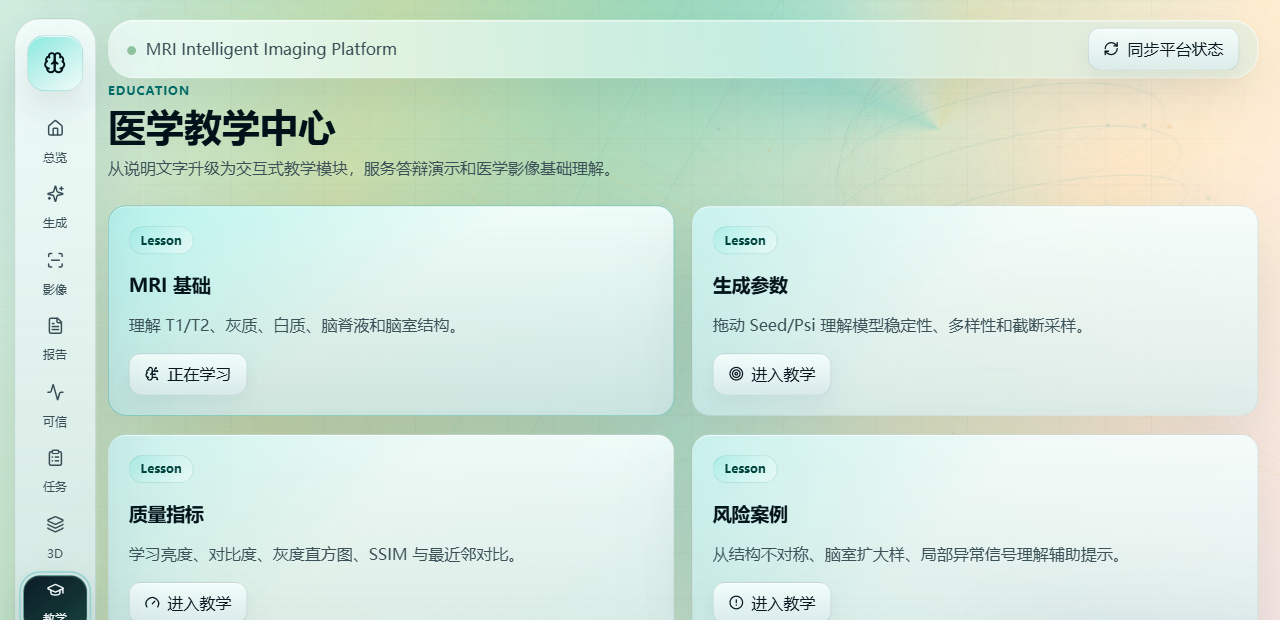
\includegraphics[width=\textwidth]{figures/frontend_education.png}
\caption{医学教学中心}
\end{subfigure}
\caption{React 前端任务管理与医学教学页面}
\label{fig:frontend-tasks-education}
\end{figure}

\section{点云初始化结果分析}
点云初始化结果由 \texttt{init\_pcd.py} 生成，输出文件为 \texttt{init\_point\_cloud.ply}。该文件大小约 13 MB。PLY 文件头显示包含 477426 个顶点，每个顶点包含三维坐标和 RGB 颜色信息。点云预览如图 \ref{fig:init-point-cloud} 所示。

\begin{figure}[H]
\centering
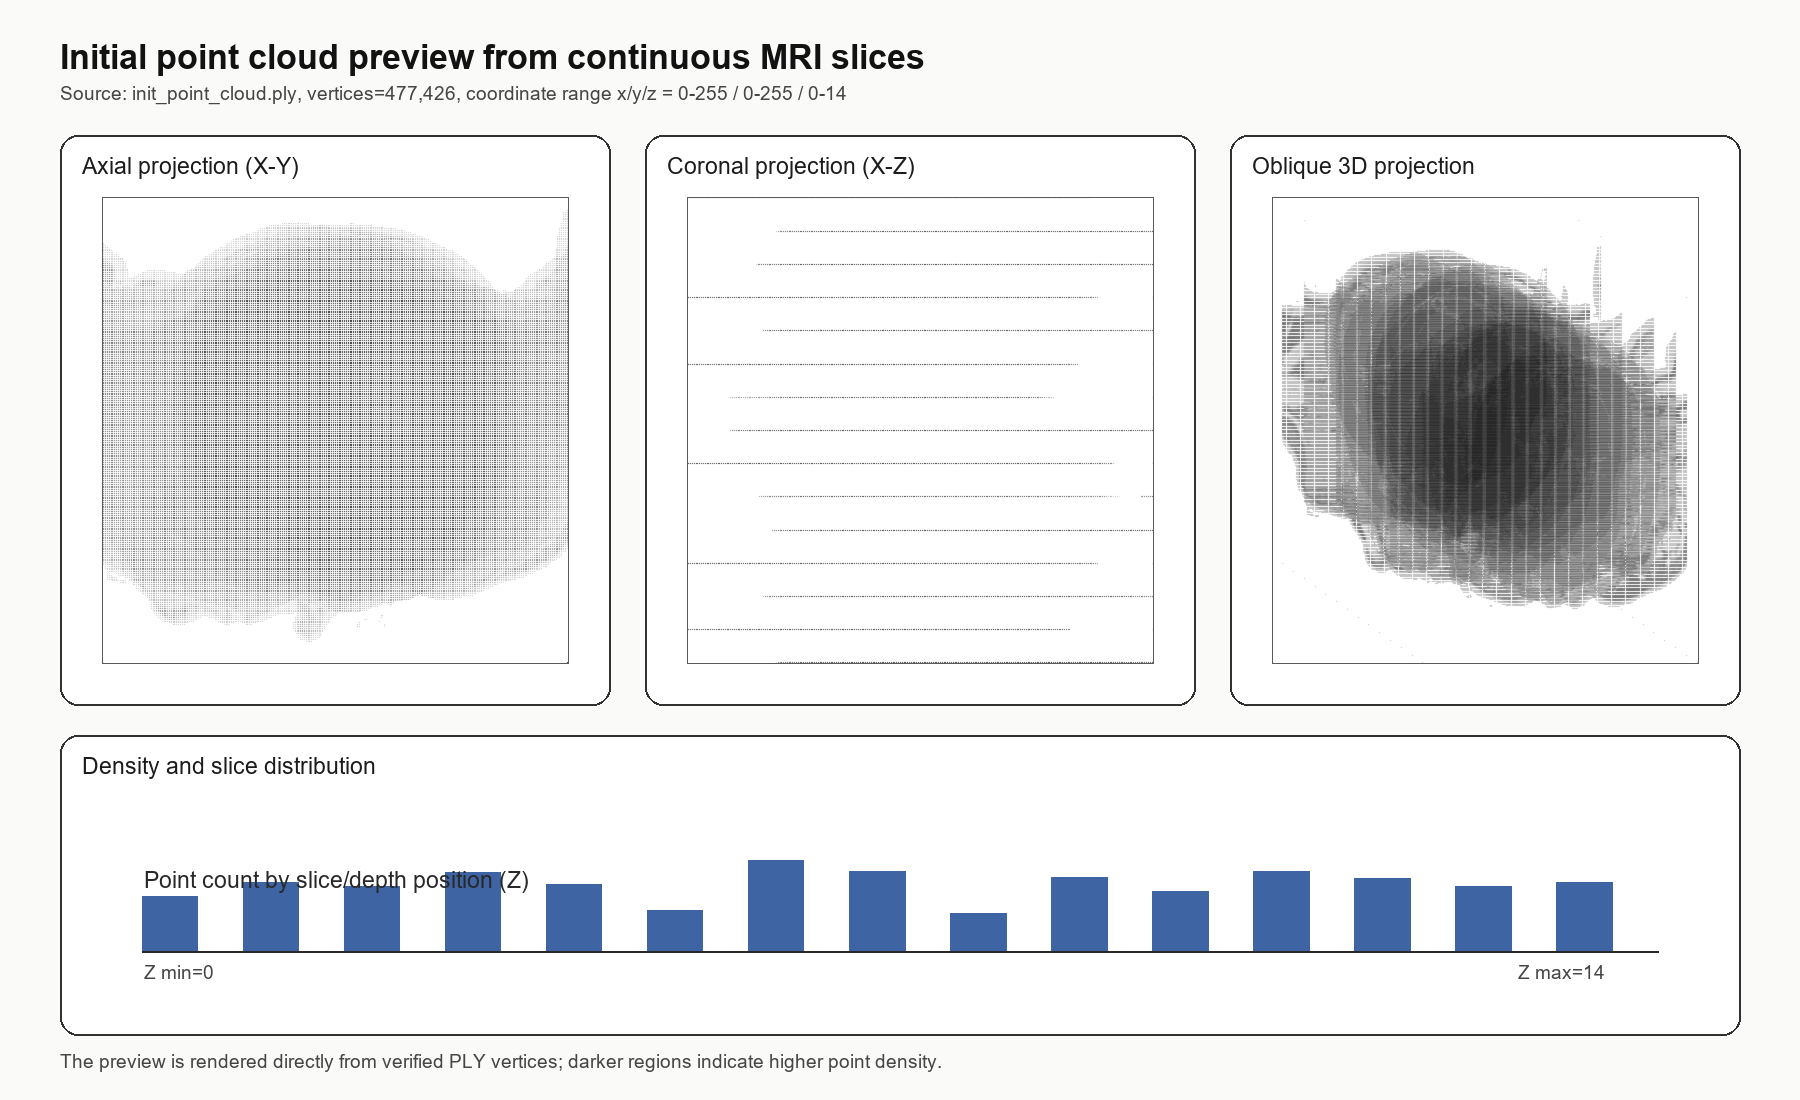
\includegraphics[width=0.82\textwidth]{figures/init_point_cloud_preview.png}
\caption{由连续 MRI 切片初始化得到的点云投影与密度分布预览}
\label{fig:init-point-cloud}
\end{figure}

该点云记录了二维切片进入三维空间的过程。每张切片对应一个 $z$ 轴位置，非背景像素被映射为空间点，像素灰度则被写入颜色强度。这样得到的点云既能作为 3DGS 三维重建输入，也能作为平台 2D/3D 对比展示的中间结果。相比只展示单张二维图，这一步提供了更明确的三维工程接口。

\section{3DGS 训练配置与重建结果}
3DGS 实验使用 180 张连续 MRI 切片作为监督图像，并以 300000 个点构建初始 PLY 点云。训练结果保存在 3DGS 主训练目录中。训练配置文件显示，模型采用三阶球谐函数表示颜色，输入图像目录为 \texttt{images}，数据设备为 CUDA。训练输出目录保存相机参数、checkpoint、训练日志、渲染结果和点云文件。

\begin{table}[H]
\centering
\caption{3DGS 训练主要参数与输出}
\begin{tabular}{>{\raggedright\arraybackslash}p{4.1cm}>{\raggedright\arraybackslash}p{8.2cm}}
\toprule
参数项 & 参数值或结果 \\
\midrule
训练切片数量 & 180 张 \\
训练图像分辨率 & $256\times256$ \\
初始点云规模 & 300000 点 \\
相机参数数量 & 180 个相机条目 \\
颜色表示 & 三阶球谐函数，\texttt{sh\_degree=3} \\
训练迭代次数 & 30000 轮 \\
最终 checkpoint & \texttt{chkpnt30000.pth} \\
最终点云 & 第 30000 轮输出 PLY 点云 \\
最终高斯点数量 & 556424 个 \\
前端预览点云 & 60000 点 \\
\bottomrule
\end{tabular}
\end{table}

训练过程中，系统在第 1000、3000、7000、15000 和 30000 轮记录训练集重建指标，也保存对应高斯点云。表 \ref{tab:3dgs-metrics} 给出了训练日志中的主要指标。随着迭代推进，L1 误差整体下降，PSNR 整体提高，说明三维高斯参数在切片监督下逐步逼近目标 MRI 切片分布。

\begin{table}[H]
\centering
\caption{3DGS 训练过程指标}
\label{tab:3dgs-metrics}
\begin{tabular}{cccc}
\toprule
迭代轮数 & L1 误差 & PSNR/dB & 说明 \\
\midrule
1000 & 0.0986 & 14.6051 & 初始优化阶段 \\
3000 & 0.0778 & 16.1066 & 结构逐步收敛 \\
7000 & 0.0675 & 16.8441 & 中期稳定优化 \\
15000 & 0.0579 & 17.9135 & 重建质量继续提升 \\
30000 & 0.0459 & 20.0909 & 最终训练结果 \\
\bottomrule
\end{tabular}
\end{table}

最新训练日志和前端展示摘要文件显示，3DGS 在第 30000 轮训练集评估中达到 L1 为 0.0459、PSNR 为 20.0909 dB。这组指标来自训练过程对 180 张监督切片的渲染重建评估，反映的是本平台实验中的重建一致性，并不能解释为医学诊断性能。训练指标变化如图 \ref{fig:3dgs-metrics-30000} 所示。

\begin{figure}[H]
\centering
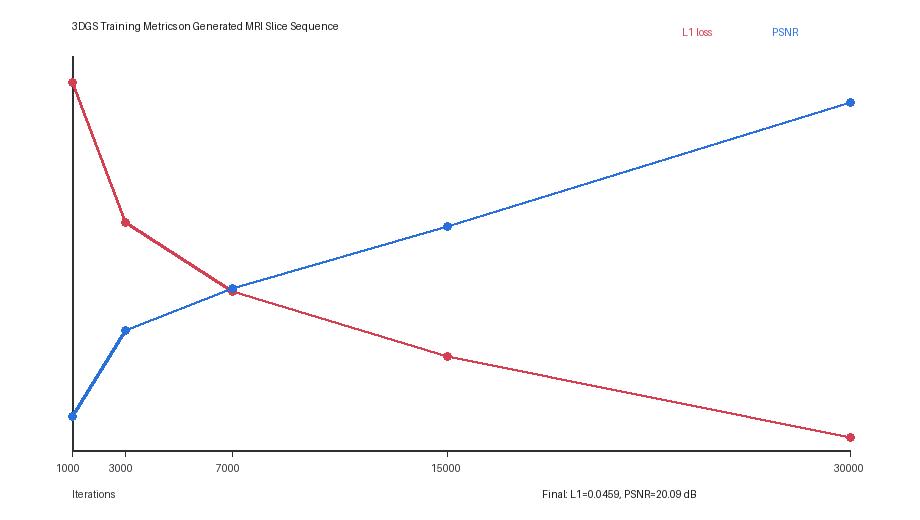
\includegraphics[width=0.9\textwidth]{figures/3dgs_metrics_30000.png}
\caption{3DGS 训练过程 L1 与 PSNR 指标变化}
\label{fig:3dgs-metrics-30000}
\end{figure}

从指标变化看，训练前期主要让整体轮廓和灰度分布逐步对齐，后期继续降低像素误差。这里的 PSNR 只说明渲染结果和监督切片之间更接近，并不能说明生成结果具备临床可用性。原因在于本实验输入是规则 MRI 切片序列，不是来自真实相机的多视角图像。本文把该指标作为工程训练过程的复核依据，而不是医学诊断性能指标。

第 30000 轮渲染切片与参考切片对比如图 \ref{fig:3dgs-comparison-30000} 所示。图中选取序列前部、中部和后部切片进行展示。渲染结果在脑部轮廓、主体灰度区域和层间变化趋势上与参考切片保持一致，但局部细节仍有一定平滑化现象。这与 MRI 灰度纹理、单序列输入约束和当前训练规模有关。

\begin{figure}[H]
\centering
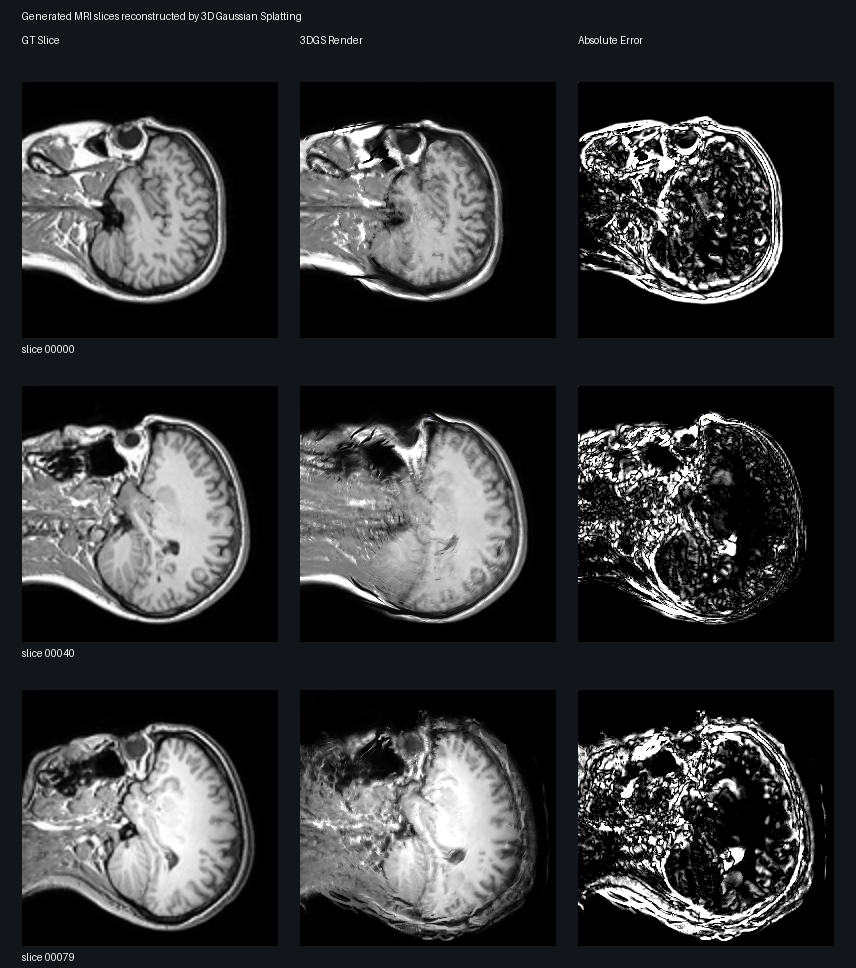
\includegraphics[width=0.82\textwidth]{figures/3dgs_slice_comparison_30000.png}
\caption{3DGS 第 30000 轮渲染切片与参考切片对比}
\label{fig:3dgs-comparison-30000}
\end{figure}

结合训练日志、checkpoint、点云文件和渲染结果可以确认，3DGS 模块已经完成训练闭环。该闭环从规则切片序列开始，最终输出可保存、可预览的三维高斯表达。输入点云从 300000 点优化为 556424 个高斯点，说明训练过程在初始空间结构基础上调整并扩展了三维表达。前端展示时，系统使用 60000 点预览点云降低浏览器加载压力，同时保留完整 PLY 文件作为实验产物。这样处理后，平台既能展示轻量化点云，也能保留完整训练结果用于复核。

\section{综合评价与局限性分析}
综合实验结果可以看到，项目已经跑通 MRI 数据预处理、StyleGAN2 二维生成、连续切片组织、点云初始化和 3DGS 三维训练结果展示等主要流程。StyleGAN2 部分留下了可加载权重和生成切片，3DGS 部分留下了训练日志、checkpoint、渲染图像和训练后点云。平台采用 FastAPI + React 架构，能够提供后端接口、前端页面、任务状态、影像查看和三维展示。就毕业设计要求而言，系统已经覆盖算法实现、工程集成、实验验证和可视化展示几个核心方面。

系统仍有可以继续改进的地方。StyleGAN2 生成结果目前主要通过可视化和工程链路验证，缺少大规模样本统计和医学专家评价。3DGS 训练基于规则切片相机和单序列灰度图像，已经能够形成可展示的三维表达，但局部组织边界仍有平滑化现象。平台目前主要以本地 FastAPI 服务和 Vite 前端运行，跨环境部署能力还可以通过统一配置、环境变量和容器化方式继续增强。
